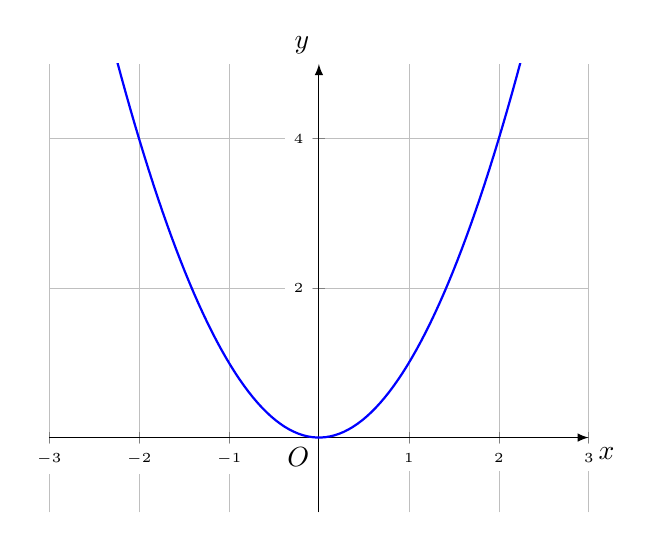
\begin{tikzpicture}
\begin{axis}[
    axis lines=middle,
    xlabel=$x$,
    ylabel=$y$,
    xmin=-3,
    xmax=3,
    ymin=-1,
    ymax=5,
    grid=both,
    grid style={line width=.1pt, draw=gray!10},
    major grid style={line width=.2pt,draw=gray!50},
    tick label style={font=\tiny,fill=white},
    axis line style={-latex},
    xlabel style={at={(ticklabel* cs:1)},anchor=north west},
    ylabel style={at={(ticklabel* cs:1)},anchor=south east}
]
\addplot[domain=-2.5:2.5, samples=100, blue, thick]{x^2};
\node[below left] at (axis cs:0,0) {$O$};
\end{axis}
\end{tikzpicture}
